% The methods that you use goes here

\footnotesize

The NSPSF is the largest remaining peatland in Peninsular Malaysia, located in northwestern Selangor near the coastal town of Sekinchan, covering ~81,304 hectares (Figure \ref{fig:map}). The land was originally logged in the 1930s and later gazetted as a protected area in the 1990s \cite{GEC_2014}. To the west lies a paddy field, part of the Tanjong Karang Irrigation Scheme, which receives drainage from the forest. Surrounding land uses include oil palm plantations, rehabilitated logging zones, and protected forest areas managed by the Selangor Forestry Department.

Entry and sampling were conducted under research permit JH/100 Jld. 31 (59), with additional approvals from the Klang and Rawang District Forestry Offices.

\begin{figure}[H]
    \vspace{-0.4cm}
    \centering
    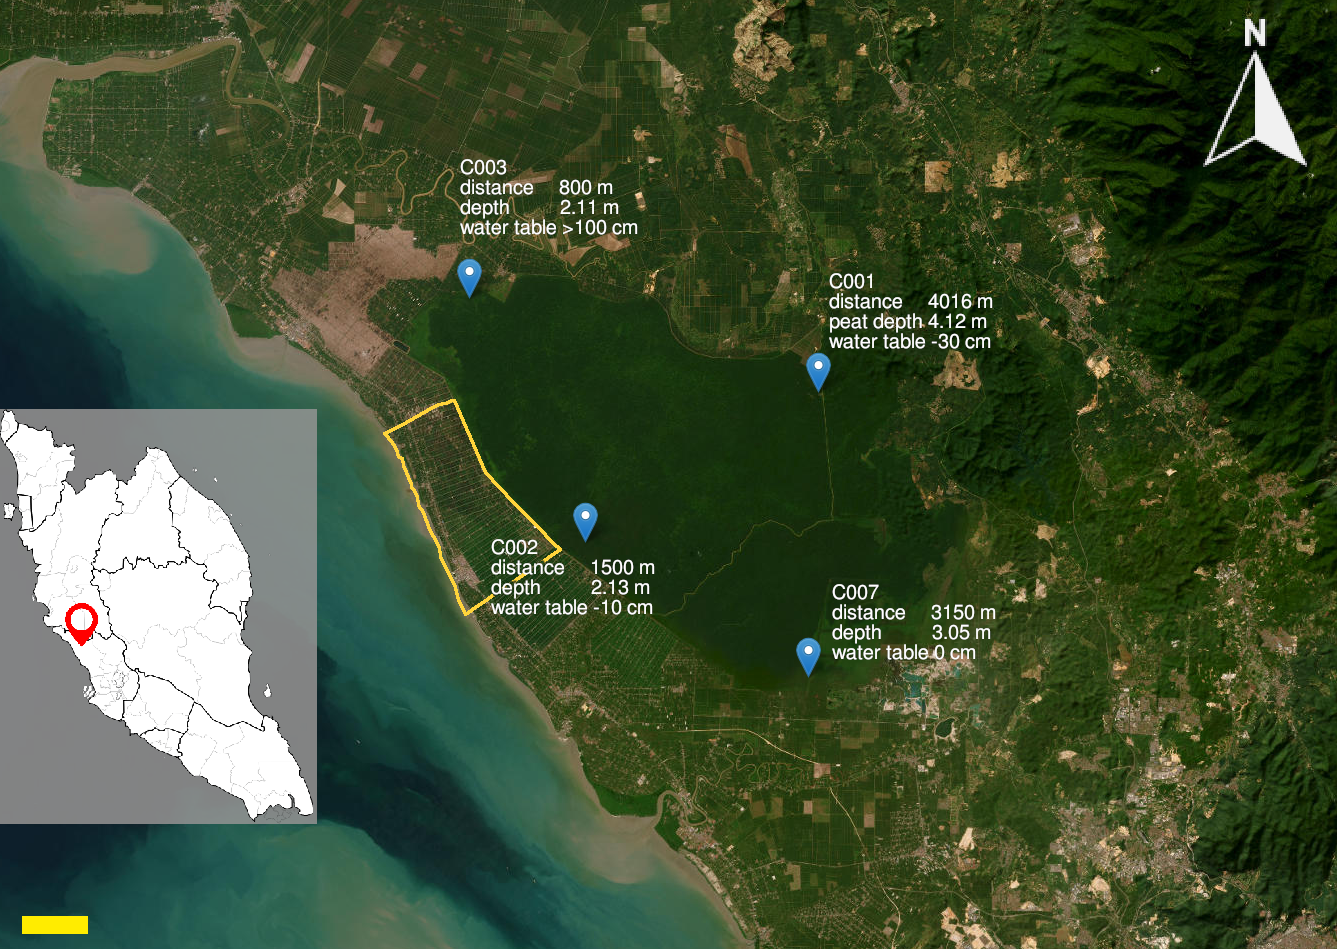
\includegraphics[width=0.9\linewidth]{content-images/map_plot4.png}
    \caption{\scriptsize Map of the NSPSF, Selangor, Peninsular Malaysia. The four sampling sites are marked with blue indicators. The scale bar in the bottom left represents a distance of 5 kilometers. The yellow boundary outlines the nearby town of Sekinchan and surrounding paddy fields. The inset map shows the location of the NSPSF (red marker) within Peninsular Malaysia.}
    \label{fig:map}
\end{figure}

\vspace{-0.3cm}

We collected 20 peat soil samples representing four contrasting NSPSF sites, each sampled at five distinct depths across the peat profile (Figure \ref{fig:map}). Genomic DNA was extracted from peat soil using a modified protocol involving cryogenic grinding, chemical lysis, and purification with chloroform:isoamyl alcohol, ethanol precipitation, and AMPure XP bead cleanups. DNA quality was evaluated via NanoDrop and Qubit. Libraries were prepared using the SQK-LSK114 ligation kit and sequenced on FLO-PRO114M flow cells with the Oxford Nanopore P2 Solo platform. We generated a minimum of 80 Gb of sequencing data per sample to ensure sufficient coverage for capturing low-abundance taxa, including methanogens.

Bioinformatics analyses were performed using the M3 MASSIVE HPC cluster (Victoria, Australia) and the Advanced Computing Platform (Monash Malaysia). The workflow is summarized in Figure \ref{fig:workflow}, and full details and workflows are available at: \url{github.com/ZarulHanifah/8thICMBB2025} \cite{Kolmogorov_2019_flye, Alneberg_2014_concoct, Pan_2022_semibin, Mallawaarachchi_2022_metacoag, Shaffer_2020_dram}.

\begin{figure}[H]
    \vspace{-0.4cm}
    \centering
    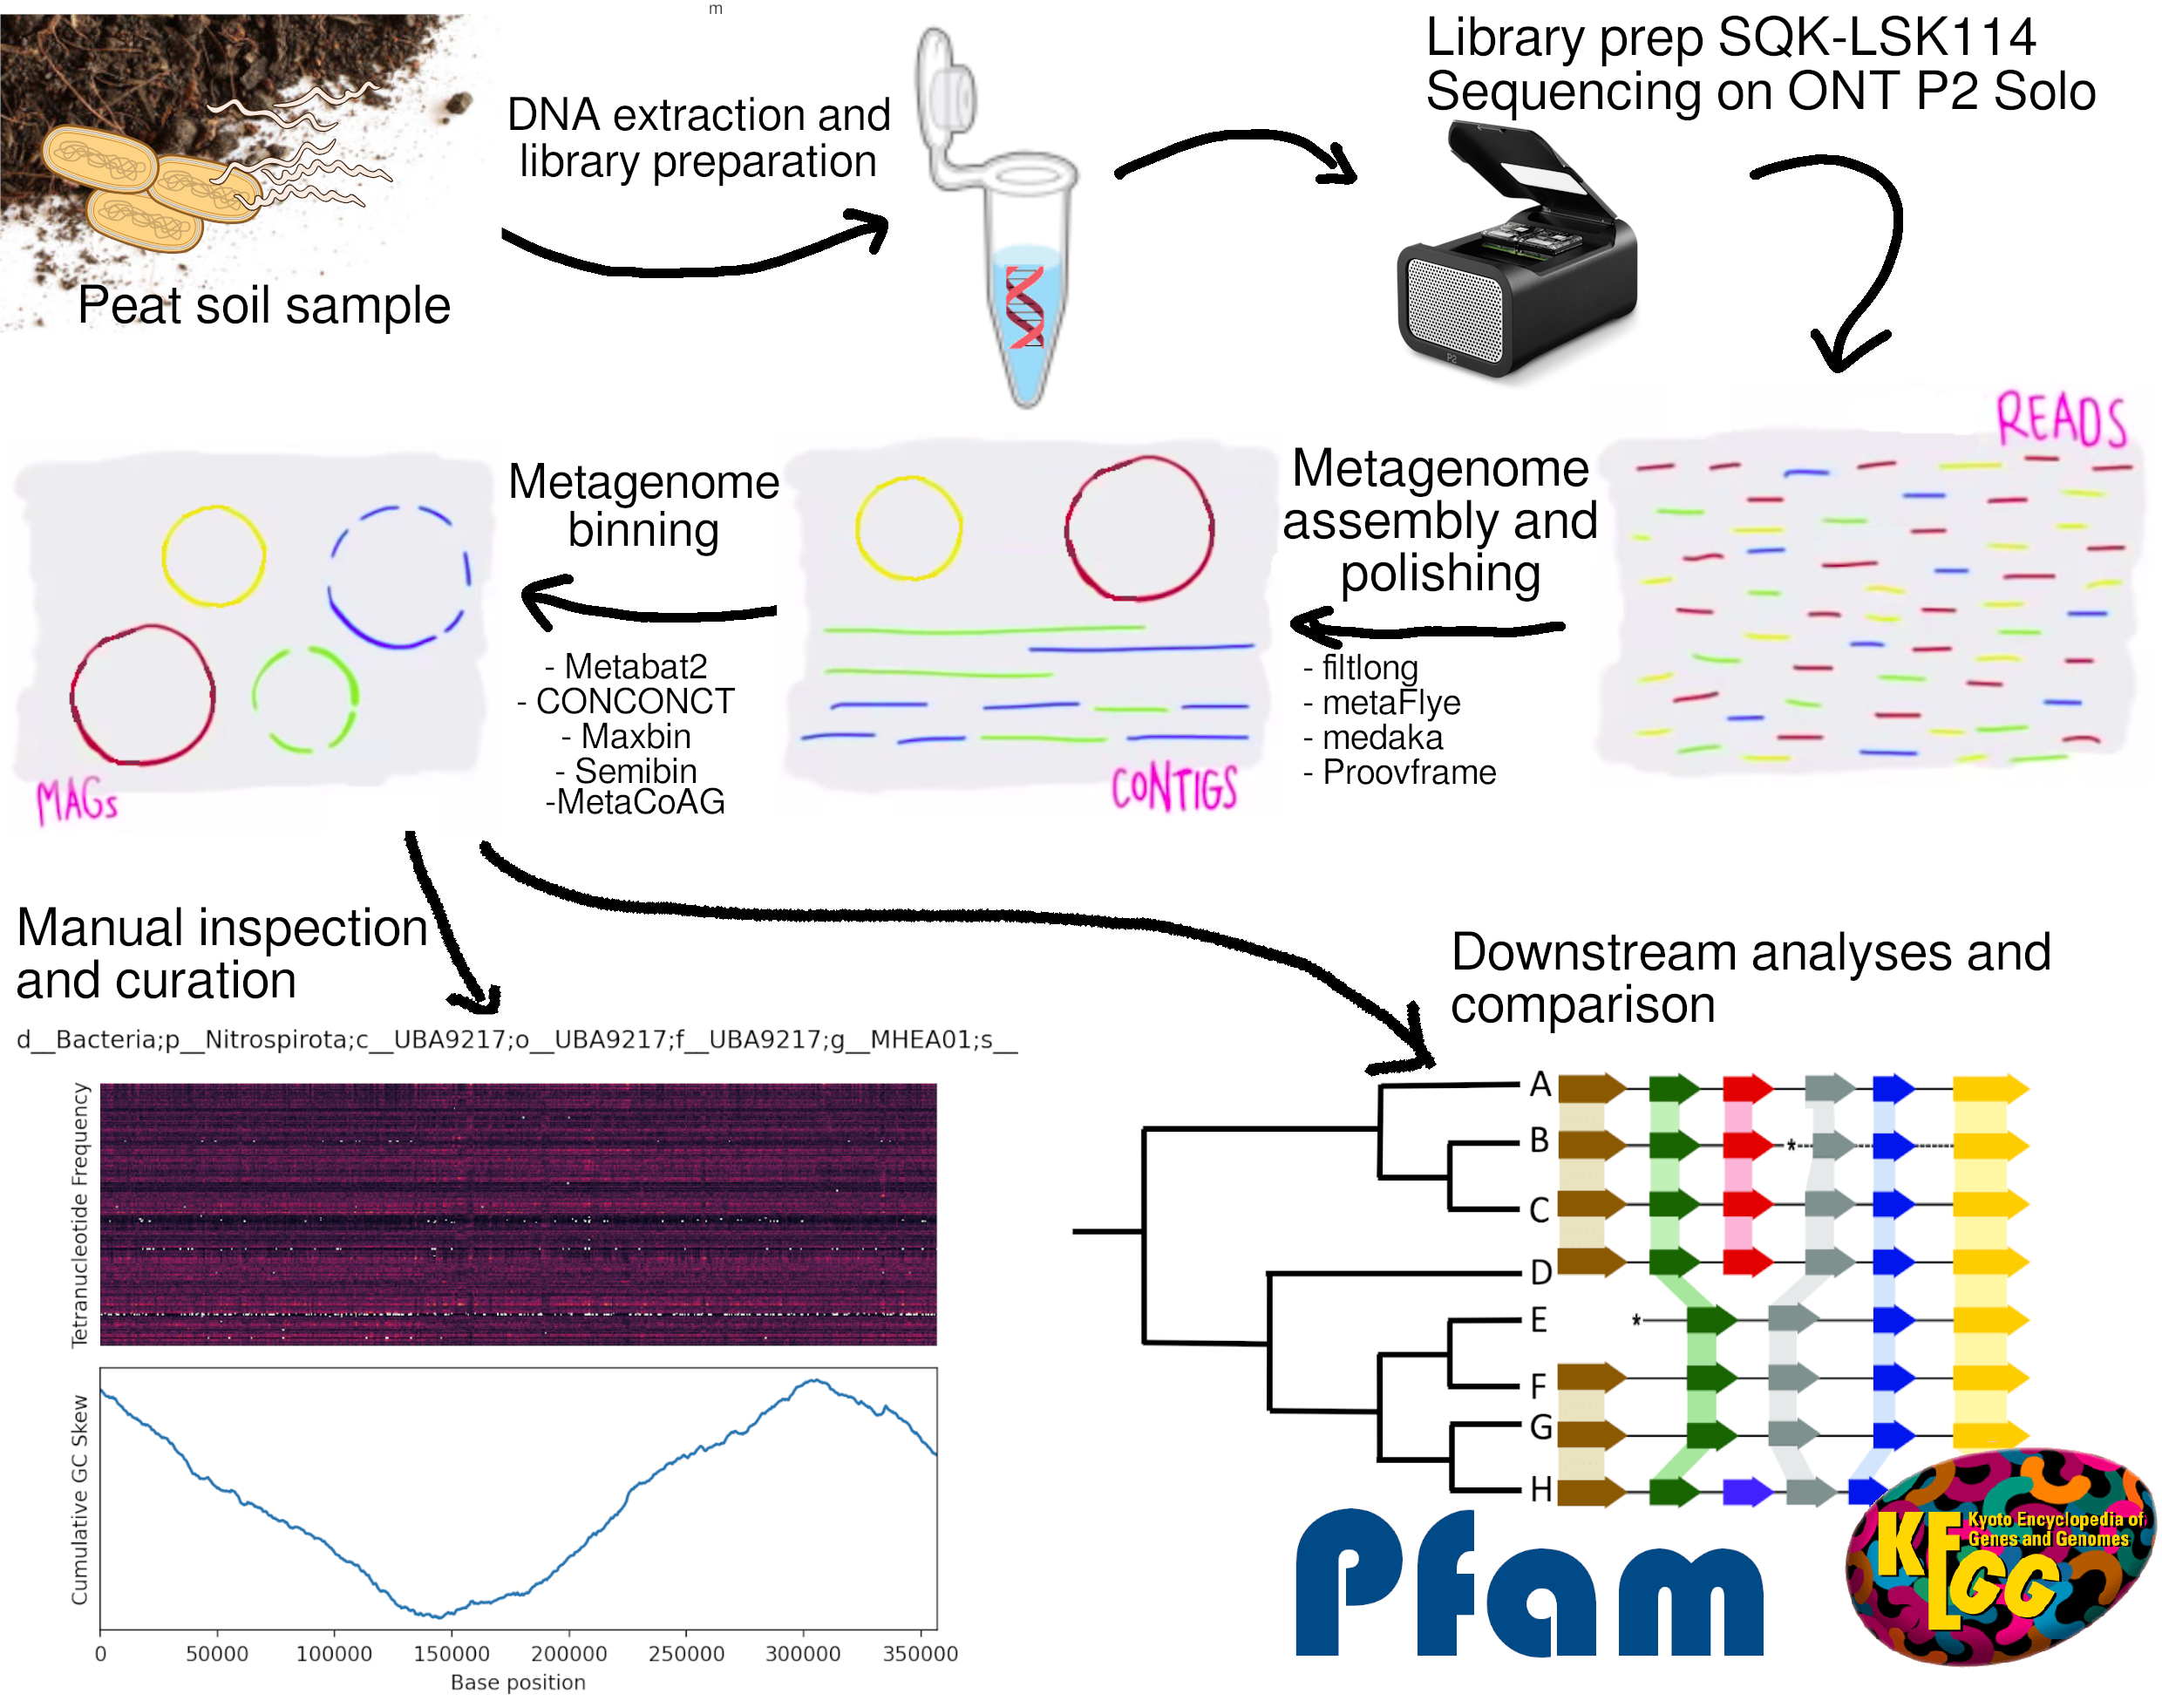
\includegraphics[width=0.9\linewidth]{experimental_design}
    \caption{\scriptsize Flowchart summarizing the workflow DNA extraction, sequencing on Oxford Nanopore P2 Solo platform and bioinformatics analyses. Manual curation and inspection included genome circulation and reorientation, and display of tetranucleotide frequency and GC skew.}
    \label{fig:workflow}
\end{figure}

% \vspace{2em} % Fill in to put references at the bottom
